\section{Theorie}
\label{sec:Theorie}
Bei diesem Versuch soll mit Hilfe der Röntgenreflektometrie die Dichte, Rauigkeit und Dicke einer Polysterolschicht 
auf einem Siliziumwafer bestimmt werden. 
Röntgenstrahlen sind elektromagnetische Wellen mit Wellenlängen im Bereich von $10^{-9}$ m bis $10^{-11}$ m.
Sie werden durch das Abbremsen von Elektronen erzeugt.

\subsection{Brechungsindex}
Trifft Röntgenstrahlung aus dem Vakuum auf eine ebene Grenzfläche, so ist der Brechungsindex des Mediums 

\begin{equation}
    n = 1- \delta + i \: \beta,
\end{equation}
dabei ist $\delta$ eine Korrektur der Größenordnung $10^{-6}$ und $\beta$ beschreibt die Absorption des Mediums.
Der Brechungsindex von Röntgenstrahlung ist kleiner als eins. Dadurch ist die äußere Totalreflektion möglich, also 
die Totalreflektion innerhalb des Vakuums.
Diese Totalreflektion findet unterhalb eines kritischen Winkels $\alpha_c$ statt.
Mit Hilfe des snelliussches Brechungsgesetzes 

\begin{equation}
    \frac{n_1}{n_2} = \frac{cos(\alpha_2)}{cos(\alpha_1)},
\end{equation}
wobei $n_1 = 1$ und $\alpha_1 = \alpha_c$,
kann der kritische Winkel zu 

\begin{equation}
    \alpha_c = \sqrt{2 \delta} = \lambda \sqrt{\frac{r_e \rho}{\pi}}
\end{equation}
bestimmt werden.
Dabei ist $r_e$ der klassische Elektronenradius, $\rho$ die Elektronendichte des Materials und $\lambda$ die Wellenlänge der Röntgenstrahlung.



\subsection{Fresnelsche Formeln}
Wenn eine ebene elektromagnetische Welle auf eine ebene Fläche trifft, beschreiben die fresnellschen Formeln das den Anteil der transmittierten und reflektierten Intensität 
im Verhältnis zur einfallenden Welle. Hierbei muss normalerweise zwischen p- und s-polarisiertem Licht unterschieden werden, doch da die Brechungsindices 
bei Röntgenstrahlung beinahe gleich sind ($n:= n_1 = n_2$), benötigt es diese Unterscheidung nicht.
Somit lauten die fresnellschen Formeln für Röntgenstrahlung

\begin{equation}
    t = \frac{2 n \cdot cos(\alpha_1)}{n \cdot cos(\alpha_1) + n \cdot cos(\alpha_2)}
\end{equation}
\begin{equation}
    r = \frac{n \cdot cos(\alpha_1) - n \cdot cos(\alpha_2)}{n \cdot cos(\alpha_1) + n \cdot cos(\alpha_2)}.
\end{equation}


\subsection{Mehrschichtsystem}
Gibt es anstatt wie bisher nicht nur eine, sondern mehrere Grenzflächen, so interferieren die von den verschiedenen grenzflächen reflektierten Wellen miteinander.
Für den einfachsten Fall mit zwei ebenen Grenzflächen kommt es dadurch zur Kiessig-Oszillation, welche in Abbildung \ref{fig:Kiessig-Oszillation} zu sehen ist.

\begin{figure}
    \centering
    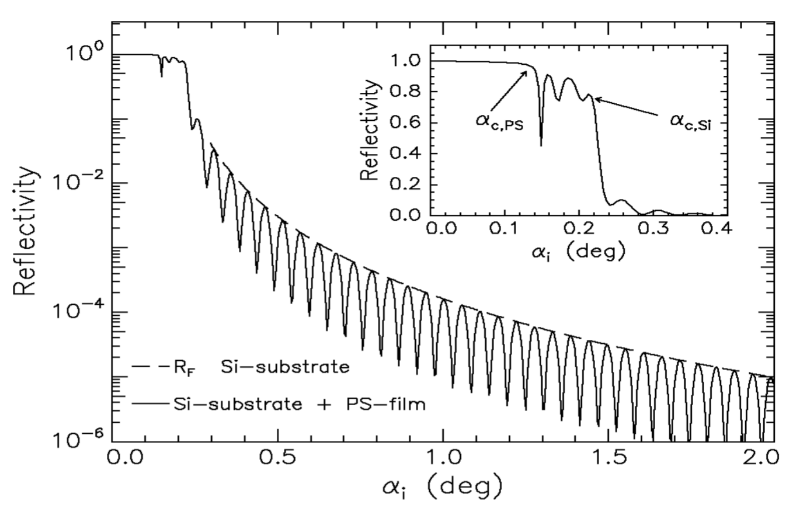
\includegraphics[width=0.6\textwidth]{Kiessig-Oszillation.png}
    \caption{Reflektivität eines Siliziumwafers mit einer 800 Å dicken Polystyrolschicht, in Abhängigkeit vom Einfallswinkel. \cite{Anleitungalt}}
    \label{fig:Kiessig-Oszillation}
\end{figure}

In diesem Fall kann die Dicke der ersten Schicht durch 

\begin{equation}
    d = \frac{\lambda}{2 \Delta \alpha_i}
\end{equation}
bestimmt werden. Dabei ist $\Delta \alpha_i$ der Abstand zweier Minima oder Maxima.
Bei mehr als zwei Grenzflächen kommt es zur überlagerung der einzelnen Kiessig-Oszillationen. 
Die Reflektivität eines solchen Systems kann dann durch den rekursiven Parratt-Algorithmus bestimmt werden.

\begin{equation}
    X_j = \frac{R_j}{T_j} = \text{exp}(-2i k_{z,j} z_j) \cdot \frac{r_{j,j+1} + X_{j+1} \text{exp}(2i k_{z,j+1} z_j) }{1 + r_{j,j+1} X_{j+1} \text{exp}(2i k_{z,j+1 z_j})}
\end{equation}
Mit $z_j$ der j-ten Grenzschicht, $r_{j,j+1}$ die Fresnelreflektivität der j-ten Grenzschicht und $k_{z,j}$ die z-Komponente des Wellenvektors in der j-ten Schicht.
Zur Berechnung wird angenommen, dass die unterste Schicht und das Vakuum unendlich weit ausgedehnt sind. Dadurch wird die von der (N+1)-ten Schicht transmittierte 
Strahlung, nicht erneut reflektiert und es gilt $R_{N+1} = X_{N+1} = 0$.
Dies ist der Startwert der Rekursion.
Werden die Oberflächen der Schichten nun nichtmehr als glatt angenommen, wird die "root-mean-square"-Rauigkeit eingeführt:

\begin{equation}
    \sigma_j^2 = \int (z - z_j)^2 \: P_j(z) dz.
\end{equation}
Dabei beschreibt $z_j$ die Position der j-ten Grenzschicht und $P_j(z)$ die Wahrscheinlichkeit, dass sich die Grenzschicht im Bereich $[z_j + z, z_j + z + dz]$ befindet.
Mit diesem anpassendem Term werden die Fresnelkoeffizienten zu 

\begin{equation}
    \tilde{r}_{j,j+1} = r_{j,j+1} \text{exp} \left(-2 k_{z,j} k_{z,j+1} \sigma_j^2\right)
\end{equation}
\begin{equation}
    \tilde{t}_{j,j+1} = t_{j,j+1} \text{exp} \left( \left(k_{z,j-k_{z,j+1}}\right)^2 \cdot \frac{\sigma_j^2}{2}\right).
\end{equation}


\subsection{Geometriefaktor}
Ist der Winkel zwischen Ausbreitungsrichtung der Röntgenstrahlung und der Grenzfläche kleiner als ein Grenzwinkel $\alpha_g$, wird für korrekte Berechnungen der sogenannte Geometriefaktor benötigt. 
Dies ist der Fall, da bei kleinen Winkeln nicht der gesamte Strahl die Probe trifft.
Der Grenzwinkel $\alpha_g$ ist gegeben durch 

\begin{equation}
    \alpha_g = arcsin \left( \frac{d_0}{D}\right),
\end{equation}
hängt also ab von der Strahlenbreite des Röntgenstrahls $d_0$ und der Länge der Probe D.
Der Geometriefaktor sieht wie folgt aus:

\begin{equation*}
    G = \left\{
        \begin{aligned}
            \frac{D \: sin(\alpha_i)}{d_0} \qquad \text{für} \: \alpha_i < \alpha_g \\
            1 \qquad \qquad \text{für} \: \alpha_i \geq \alpha_g
        \end{aligned}
        \right
\end{equation*}



